% !TEX program = pdflatex
\documentclass[3p,11pt]{elsarticle}
\usepackage{amsmath,amssymb}
\usepackage{array}
\usepackage{booktabs}
\usepackage[tableposition=top]{caption}
\usepackage{graphicx}
\usepackage{url}
\urlstyle{same}
\usepackage[hidelinks]{hyperref}
\emergencystretch=3em
% first-page footer: the page number alone
\makeatletter
\def\ps@pprintTitle{\let\@oddhead\@empty\let\@evenhead\@empty
  \def\@oddfoot{\hfil\thepage\hfil}\let\@evenfoot\@oddfoot}
\makeatother

% ---- notation ---------------------------------------------------------------
\newcommand{\kms}{km\,s$^{-1}$}
\newcommand{\ms}{m\,s$^{-1}$}
\newcommand{\Msun}{M$_\odot$}
\newcommand{\Rsun}{R$_\odot$}
\newcommand{\Lsun}{L$_\odot$}
\newcommand{\Mearth}{M$_\oplus$}
\newcommand{\Rearth}{R$_\oplus$}

\begin{document}

\begin{frontmatter}

\title{HD\,71334\,b: a Neptune-mass planet on an 89-day orbit around an old solar analogue, in public
HARPS and Keck velocities}

\author{Charles C. Norton}

\begin{abstract}
HD\,71334 (GJ\,9263, HIP\,41317) is a G2.5 dwarf of 0.93\,\Msun\ at 39.2\,pc, about 10\,Gyr old,
slightly metal-poor and magnetically quiet. Its public velocities, from HARPS on 67 nights between 2003
and 2017 and from Keck's HIRES on 34 nights between 1997 and 2019, carry a Keplerian signal at
88.91\,d with a semi-amplitude of 3.0\,\ms: a planet of at least 20\,\Mearth\ at 0.38\,au,
HD\,71334\,b. The signal stands in three reductions of the HARPS spectra, SERVAL's
velocities, the HARPS pipeline's and line-by-line velocities measured here, at false-alarm levels of
$10^{-10}$, $2\times10^{-8}$ and $2\times10^{-5}$, keeps its amplitude and phase from the first half
of the nights to the second in each, and appears in the Keck velocities, most of them taken before
HARPS began, at $2.0 \pm 0.4$\,\ms\ with the HARPS phase held. Its one-year aliases at 71.5 and
117.2\,d fit worse by 22 and 27 in log-likelihood, and no simulation of the observing window with
the planet at either alias reproduces the observed periodogram. No activity indicator has power at
the period, and the orbit is consistent with circular. The archive's one-dimensional spectra of twelve
nights were wavelength-calibrated with a ThAr exposure taken 196 to 530 days earlier, and on those
nights line-by-line velocities stand up to 9\,\ms\ from SERVAL's; left in, they move the line-by-line
periodogram's highest peak to the one-year alias. TESS's five sectors all fall between the planet's
predicted conjunctions, so whether it transits, with a probability of 1.3 per cent, is open, and the
conjunction times are given for photometry.
\end{abstract}

\begin{keyword}
Techniques: radial velocities \sep Planets and satellites: detection \sep Stars: individual: HD\,71334
\end{keyword}

\end{frontmatter}

\section{Introduction}\label{sec:intro}

Planets of ten to thirty Earth masses on orbits of weeks to months are among the commonest that
radial-velocity surveys of Sun-like stars find~\cite{Howard2010}. Their velocity signals, a few metres
per second, sit at the level that several years of a stable spectrograph resolve, and the public archives
now hold such records for hundreds of nearby stars. HARPS-RVBank~\cite{Trifonov2020} recomputed every
public HARPS velocity with SERVAL~\cite{Zechmeister2018}, corrected the instrument's nightly zero
points and attached each spectrum's activity indicators, the California Legacy
Survey~\cite{Rosenthal2021} released three decades of Keck HIRES velocities, and DACE serves the HARPS
pipeline's own velocities beside the Keck ones.

HD\,71334 is in both surveys. HARPS observed it on 67 nights between 2003 and 2017 and HIRES on 34
between 1997 and 2019, and no planet has been reported around it. Its velocities carry one: a planet
of at least 20 Earth masses on an 89-day orbit, HD\,71334\,b, which we call Magrathea, after the
planet-building world of Douglas Adams's \emph{The Hitchhiker's Guide to the
Galaxy}~\cite{Adams1979}.\footnote{The planet-interior code MAGRATHEA~\cite{Huang2022} shares the
name.}
Section~\ref{sec:data} describes the data, Section~\ref{sec:star} the star, Section~\ref{sec:signal}
the signal and its aliases, Section~\ref{sec:tests} the tests against the instrument and stellar
activity, Section~\ref{sec:orbit} the orbit and the mass, Section~\ref{sec:tess} TESS's photometry, and
Section~\ref{sec:discussion} the planet.

\section{Data}\label{sec:data}

HARPS-RVBank holds 67 velocities of HD\,71334, one a night, from 2003 December 14 to 2017 February
25, with a median error of 0.83\,\ms; eight nights follow HARPS's fibre upgrade of 2015
June~\cite{LoCurto2015}, across which the velocities take an offset of their own. The same spectra give
two further sets of velocities. DACE holds the HARPS pipeline's cross-correlation velocities, 65 nights
after quality control and cleaning, with the Mount Wilson S index of each spectrum. The third set was
measured here from the ESO Science Archive's HARPS spectra, the one of highest signal to noise from
each of 69 nights, two of them in 2023 May: every spectrum is put on a grid uniform in log wavelength
at 0.4\,\kms\ from 3800 to 6880\,\AA\ in the star's frame, the median spectrum is the template, and
each spectrum's shift in each of the template's 3\,769 lines deeper than 4 per cent is Bouchy's
derivative estimate~\cite{Bouchy2001} with its photon error. A spectrum's velocity is the weighted mean
of its lines, lines more than $5\sigma$ from the median set aside and each line carrying a jitter of its
own, in the manner of line-by-line velocimetry~\cite{Artigau2022}. Each line's shifts are correlated
with the S index measured in the same spectra, and the 86 lines whose correlation passes $p < 0.01$ are
left out of a second velocity, made from the 3\,683 quiet lines. Each spectrum's header names the ThAr
exposure that set its wavelengths, which Section~\ref{sec:tests} uses.

The California Legacy Survey's HIRES velocities of HD\,71334 number 36, from 34 nights between 1997
January 13 and 2019 January 25, 27 of them before HIRES's detector upgrade of 2004 August and seven
after, with a median error of 1.45\,\ms; each era takes an offset of its own. The activity indicators are
the bank's chromatic index, differential line width, H$\alpha$ and Na\,D indices and the pipeline's
line width and bisector, and the S index from DACE and from the line-by-line spectra. The star's TESS
light curves~\cite{Ricker2015}, sector 8 (2019 February), sectors 34 and 35 (2021 January to March) at
two-minute cadence and sectors 61 (2023 January) and 88 (2025 January) at 20-second cadence, all from
SPOC, come through Lightkurve~\cite{Lightkurve2018}.

\section{The star}\label{sec:star}

Table~\ref{tab:star} gives the star's parameters. Gaia DR3~\cite{GaiaDR3} places it at
$39.23 \pm 0.03$\,pc with a renormalised unit weight error of 0.99 and no non-single-star solution, and
its astrophysical parameters~\cite{Creevey2023} give a G dwarf of 5\,630\,K, $[\mathrm{M/H}] = -0.09$,
0.93\,\Msun, 1.05\,\Rsun\ and 0.99\,\Lsun, 10.4\,Gyr old; Gaia's spectroscopic parameters give
5\,657\,K and $[\mathrm{M/H}] = -0.15$. The S index of its 67 HARPS spectra has a median of 0.167,
$\log R'_\mathrm{HK} = -4.95$ for $B-V = 0.643$~\cite{Noyes1984}, the activity of a quiet, slowly
rotating star; the activity-rotation relation~\cite{Mamajek2008} gives a rotation period near 24\,d. No
star within 2$^\circ$, 1.4\,pc at its distance, shares its parallax and proper motion.

\begin{table}[!htbp]
\centering
\caption{HD\,71334.}\label{tab:star}
\begin{tabular}{l r l}
\toprule
Parameter & Value & Source \\
\midrule
Gaia DR3 & 5644325284591298688 & \cite{GaiaDR3} \\
$G$, $G_\mathrm{BP} - G_\mathrm{RP}$ (mag) & 7.65, 0.83 & \cite{GaiaDR3} \\
$V$, $B-V$ (mag) & 7.82, 0.643 & \cite{vanLeeuwen2007} \\
Parallax (mas) & $25.490 \pm 0.017$ & \cite{GaiaDR3} \\
RUWE & 0.99 & \cite{GaiaDR3} \\
$T_\mathrm{eff}$ (K) & 5\,630 & \cite{Creevey2023} \\
$\log g$ & 4.34 & \cite{Creevey2023} \\
$[\mathrm{M/H}]$ & $-0.09$ & \cite{Creevey2023} \\
Mass (\Msun) & $0.927 \pm 0.040$ & \cite{Creevey2023} \\
Radius (\Rsun) & $1.047 \pm 0.021$ & \cite{Creevey2023} \\
Luminosity (\Lsun) & $0.993 \pm 0.005$ & \cite{Creevey2023} \\
Age (Gyr) & $10.4^{+1.3}_{-1.3}$ & \cite{Creevey2023} \\
S index & 0.167 & HARPS, DACE \\
$\log R'_\mathrm{HK}$ & $-4.95$ & this work \\
\bottomrule
\end{tabular}
\end{table}

\section{The signal}\label{sec:signal}

\subsection{Periodograms}

A generalised Lomb-Scargle periodogram~\cite{Zechmeister2009} of SERVAL's nightly velocities from 1.2 to
3\,000\,d, the offset across the fibre upgrade fitted, peaks at 88.96\,d at a false-alarm
level~\cite{Baluev2008} of $10^{-10}$. Joined to the HIRES velocities, each era with its own offset and
each telescope with its own jitter, the 101 nights over 22 years peak at 88.92\,d at
$3\times10^{-8}$; with that signal's sinusoid fitted, the residuals' highest peak, at 40.7\,d, stands at
0.39 (Figure~\ref{fig:periodograms}).

\begin{figure}[!htbp]
\centering
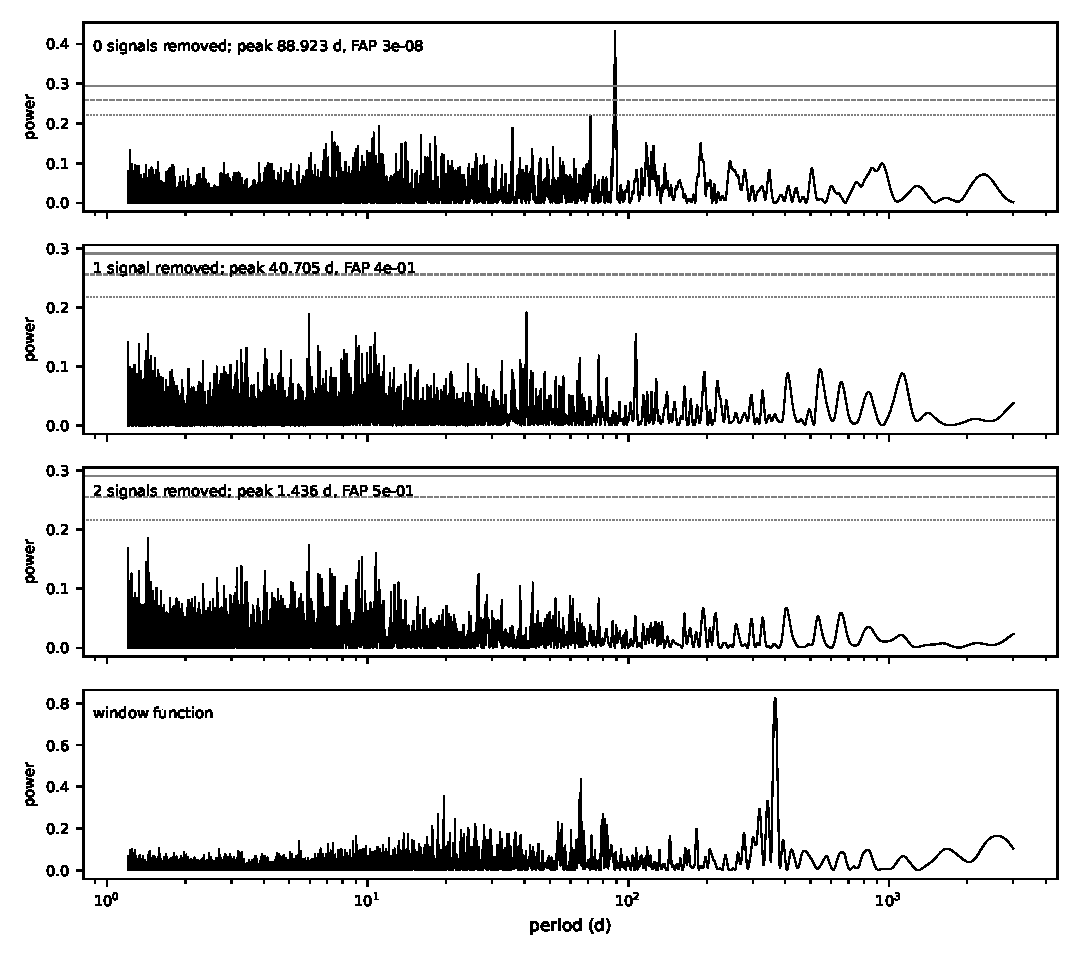
\includegraphics[width=0.92\textwidth]{periodograms.pdf}
\caption{Generalised Lomb-Scargle periodograms of the nightly HARPS and HIRES velocities of HD\,71334,
each with the sinusoids of the signals above it fitted jointly, and the observing window's spectral
window at the bottom. The horizontal lines are the false-alarm levels of 0.1, 0.01 and
0.001.}\label{fig:periodograms}
\end{figure}

\subsection{Models}

Models with no planet, with the planet and with a second one at the residuals' highest peak were
fitted by least squares, each with an offset for each era of each telescope and each telescope's
jitter added to its errors (Table~\ref{tab:models}). The planet lowers the Bayesian information
criterion~\cite{Schwarz1978} by 57.3 with a circular orbit. A free eccentricity improves the
log-likelihood by 2.1 for two more parameters and raises the BIC by 4.9, so the circular orbit is
preferred. HARPS's velocities alone give the same: the planet lowers their BIC by 57.9.

\begin{table}[!htbp]
\centering
\caption{Models of the HARPS and HIRES velocities of HD\,71334: log-likelihood with free and with
circular orbits, the Bayesian information criterion of each, and each telescope's jitter in the free
model.}
\label{tab:models}
\small
\begin{tabular}{l r r r r r r}
\toprule
Periods & $\ln L$ & $\ln L$ (circular) & BIC & BIC (circular) & Jitter, HARPS & Jitter, HIRES \\
& & & & & (\ms) & (\ms) \\
\midrule
None & $-254.9$ & $-254.9$ & 537.5 & 537.5 & 2.49 & 3.69 \\
88.9\,d & $-217.2$ & $-219.3$ & 485.1 & 480.2 & 1.24 & 3.67 \\
88.9 and 40.7\,d & $-203.6$ & $-207.6$ & 481.0 & 470.6 & 0.91 & 3.47 \\
\bottomrule
\end{tabular}
\end{table}

\subsection{Aliases}

The observing window of a star seen each year from the same season puts aliases at
$|1/P \pm 1/\mathrm{yr}|$, whose peaks in the joint periodogram lie at 71.5 and 117.2\,d (the daily
aliases lie near one day, below the periods searched). They carry 0.237 and 0.209 of the periodogram's
power against 0.553 at 88.9\,d, and the circular model refitted with the planet at either alias loses
22.4 and 26.6 in log-likelihood. The observing window decides as well~\cite{Dawson2010}. Three hundred
sets of velocities drawn at the observed times from the circular model with the fitted jitters, with
the planet at 88.9\,d, give a ratio of the powers at 88.9 and 71.5\,d of $1.88^{+0.32}_{-0.25}$, and
10 per cent of them reach the observed 2.33; three hundred with the planet at 71.5\,d give
$0.68^{+0.09}_{-0.08}$, and none reaches it. Against 117.2\,d the observed ratio, 2.66, lies above
every simulation of both kinds, those with the planet at 88.9\,d giving $1.68^{+0.29}_{-0.19}$ and
those with it at 117.2\,d $0.46^{+0.08}_{-0.09}$. HARPS's velocities alone give the same verdict, the
refits at the two aliases losing 25.3 and 25.5 in log-likelihood. The period is 88.9\,d.

\section{The instrument and stellar activity}\label{sec:tests}

\subsection{Three reductions}

Table~\ref{tab:reductions} gives the signal in each of the three reductions of the HARPS spectra, with
its semi-amplitude fitted to the first and to the second half of the nights apart. SERVAL fits a
template to every spectrum's whole extracted orders, the pipeline cross-correlates a binary mask, and
the line-by-line velocities weigh each line by its own scatter, so a signal one reduction made would not
stand in the others. The signal stands in all three as the highest peak of the periodogram, keeps its
phase from one half of the nights to the other in each, and stands at the same strength in the
velocities of the 3\,683 lines whose shifts do not follow the S index as in those of all 3\,769, as it
would not if the activity-sensitive lines carried it.

\begin{table}[!htbp]
\centering
\caption{The 88.9-day signal of HD\,71334 in three reductions of its HARPS spectra: the periodogram's
highest peak, its false-alarm level, and the semi-amplitude in the first and second half of the
nights.}\label{tab:reductions}
\begin{tabular}{l r r r r}
\toprule
Reduction & Nights & Peak (d) & False alarm & $K$ in each half (\ms) \\
\midrule
SERVAL & 67 & 88.96 & $1.0\times10^{-10}$ & $2.84 \pm 0.37$, $3.66 \pm 0.49$ \\
Pipeline & 65 & 88.63 & $1.9\times10^{-8}$ & $2.21 \pm 0.45$, $3.32 \pm 0.54$ \\
Line-by-line, all lines & 57 & 89.00 & $2.1\times10^{-5}$ & $3.12 \pm 0.56$, $4.21 \pm 0.71$ \\
Line-by-line, quiet lines & 57 & 89.00 & $4.3\times10^{-5}$ & $3.01 \pm 0.56$, $4.16 \pm 0.71$ \\
\bottomrule
\end{tabular}
\end{table}

The line-by-line velocities in Table~\ref{tab:reductions} leave out twelve nights. The pipeline sets
each spectrum's wavelengths from a ThAr exposure, as a rule from the same night, and corrects its own
velocities for the spectrograph's drift since that exposure, measured in the simultaneous reference
fibre. The archive's spectra of 2012 April 30 and May 1 and of 2013 January 6 to 9 and March 24 to 30
were calibrated with the ThAr exposure of 2011 October 16, taken 196 to 530 days before them, and on
those nights the line-by-line velocities differ from SERVAL's by $-9.5$ to $+6.4$\,\ms, a median of
$-7.1$\,\ms\ (Figure~\ref{fig:calibration}). On the 47 nights before the fibre upgrade calibrated within
ten days, the two differ by 1.6\,\ms\ in scatter and by at most 4.1\,\ms. With the twelve nights in, the
line-by-line velocities' jitter rises from 1.8 to 3.1\,\ms\ and their periodogram's highest peak moves
to 71.5\,d, the one-year alias, a few runs of large offsets standing in for the planet.

\begin{figure}[!htbp]
\centering
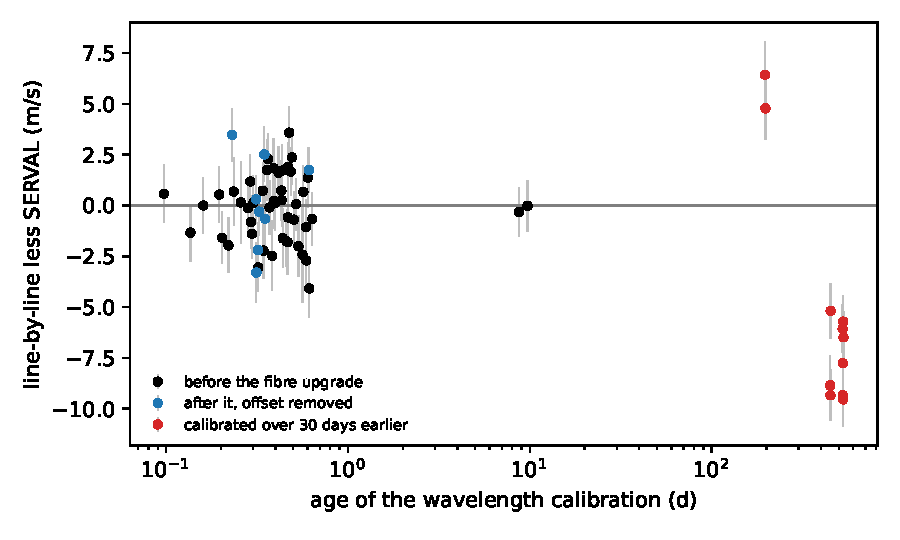
\includegraphics[width=0.75\textwidth]{calibration.pdf}
\caption{Line-by-line velocities of HD\,71334 less SERVAL's, night by night, against the age of the
ThAr exposure that set each spectrum's wavelengths. The nights after the fibre upgrade are shown with
their offset removed.}\label{fig:calibration}
\end{figure}

\subsection{Activity indicators}

The periodograms of the chromatic index, the differential line width, the H$\alpha$ and Na\,D indices,
the pipeline's line width and bisector and the S index from DACE's spectra and from the line-by-line
spectra have no power at 88.9\,d: within 5 per cent of it, the highest peak of the H$\alpha$ index stands
at a false-alarm level of 0.55 and every other indicator's at 1.0. Their own highest peaks lie at
16.0\,d (the chromatic index, $7\times10^{-3}$), at 181\,d, close to half a year (H$\alpha$,
$9\times10^{-6}$), at the longest periods searched (the two line widths, $10^{-18}$ and
$4\times10^{-6}$) and nowhere significant (Na\,D, the bisector and both S indices). The star's rotation, near 24\,d, matches neither the period
nor its harmonics.

\subsection{Keck}

Fitted at 88.89\,d with their own offsets, the 34 HIRES nights give a semi-amplitude of
$2.2 \pm 0.4$\,\ms\ at a phase $19 \pm 8^\circ$ from HARPS's, and $2.0 \pm 0.4$\,\ms\ with HARPS's phase
held; with a jitter of 2\,\ms\ added to their errors, $1.9 \pm 0.7$ and $1.8 \pm 0.7$\,\ms. Twenty-six
of the 34 nights precede HARPS's first velocity of the star, so a different telescope with a different
calibration, a decade earlier, sees the same orbit at a consistent amplitude.

\subsection{The residual at 40.7 days}

The joint residuals' highest peak, at 40.7\,d, lowers the BIC by 9.6 with a circular orbit, but its
periodogram peak stands at a false-alarm level of 0.39, which counts the search over periods that the
BIC does not. In SERVAL's velocities alone it stands at 0.05 and lowers the BIC by 17.1, and HIRES
gives $1.7 \pm 0.4$\,\ms\ at SERVAL's phase; but the pipeline's and the line-by-line velocities, with
the planet fitted, have no peak near it (false-alarm levels of 1.0), and the chromatic index, which
follows the colour of spots, has power near it at a false-alarm level of 0.1. It is not claimed.

\section{Orbit and mass}\label{sec:orbit}

Table~\ref{tab:orbit} gives the orbit, sampled with emcee~\cite{ForemanMackey2013} and its
differential-evolution moves~\cite{terBraak2006} from the 101 nights, 48 walkers over 20\,000 steps,
with an offset for each era of each telescope, each telescope's jitter and the orbit held circular.
Sampled with its eccentricity free, the orbit keeps its period and semi-amplitude within their errors,
and the eccentricity, $0.15 \pm 0.09$, lies below 0.29 at 95 per cent; a median above zero is what noise
gives a quantity that cannot be negative~\cite{Lucy1971}. Figure~\ref{fig:phased} shows the velocities
phased at the period.

\begin{table}[!htbp]
\centering
\caption{HD\,71334\,b: medians and 68 per cent intervals of the circular orbit sampled from the HARPS
and HIRES velocities, with the star's mass of 0.927\,\Msun; the eccentricity's bound is from the orbit
sampled with it free.}
\label{tab:orbit}
\begin{tabular}{l r}
\toprule
Parameter & Value \\
\midrule
Period (d) & $88.910 \pm 0.067$ \\
Semi-amplitude $K$ (\ms) & $3.03 \pm 0.27$ \\
Time of conjunction (BJD) & $2455933.26 \pm 1.17$ \\
Eccentricity & $< 0.29$ (95 per cent) \\
Minimum mass $m \sin i$ (\Mearth) & $20.1 \pm 1.8$ \\
Semi-major axis (au) & 0.380 \\
Insolation (Earth's) & 6.9 \\
Equilibrium temperature, no albedo (K) & 451 \\
Transit probability & 1.3 per cent \\
Jitter, HARPS (\ms) & $1.38^{+0.17}_{-0.15}$ \\
Jitter, HIRES (\ms) & $3.88^{+0.59}_{-0.50}$ \\
\bottomrule
\end{tabular}
\end{table}

\begin{figure}[!htbp]
\centering
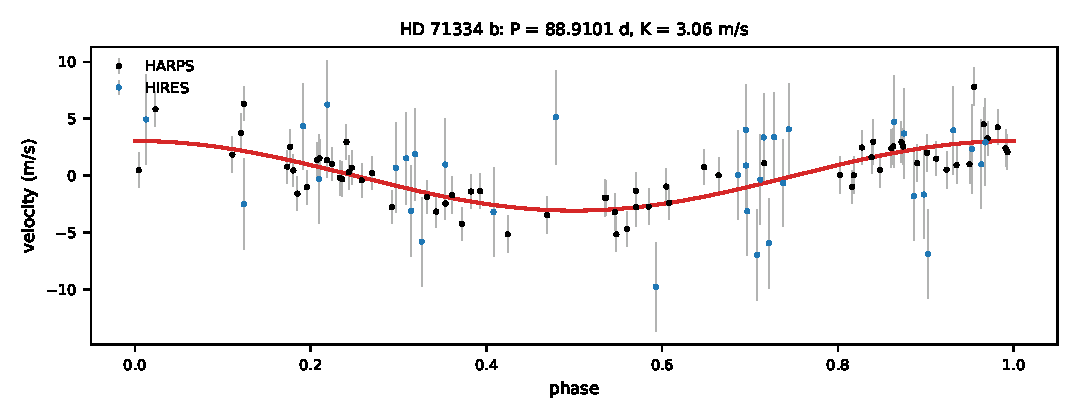
\includegraphics[width=0.95\textwidth]{phased.pdf}
\caption{The nightly velocities of HD\,71334 from HARPS (black) and HIRES (blue), each era's offset
removed, phased at 88.91\,d with the circular orbit. The error bars include each telescope's
jitter.}\label{fig:phased}
\end{figure}

The residuals of the circular orbit bound what else the velocities hold (Figure~\ref{fig:limits}). A
circular orbit is recovered 90 per cent of the time at a semi-amplitude of 2.4\,\ms\ out to 160\,d, a
minimum mass of 4 to 5\,\Mearth\ at 1.5 to 3\,d, 7\,\Mearth\ at 7\,d, 10\,\Mearth\ at 23\,d,
13\,\Mearth\ at 50\,d and 20\,\Mearth\ at 160\,d; at 2.4 to 3.1\,\ms\ from 200 to 770\,d, 24 to
43\,\Mearth, except near a year, where the seasons' gaps raise it to 55\,\Mearth. Beyond 1\,700\,d, where the four
eras' offsets absorb an orbit, no semi-amplitude up to 15\,\ms\ is recovered 90 per cent of the time.

\begin{figure}[!htbp]
\centering
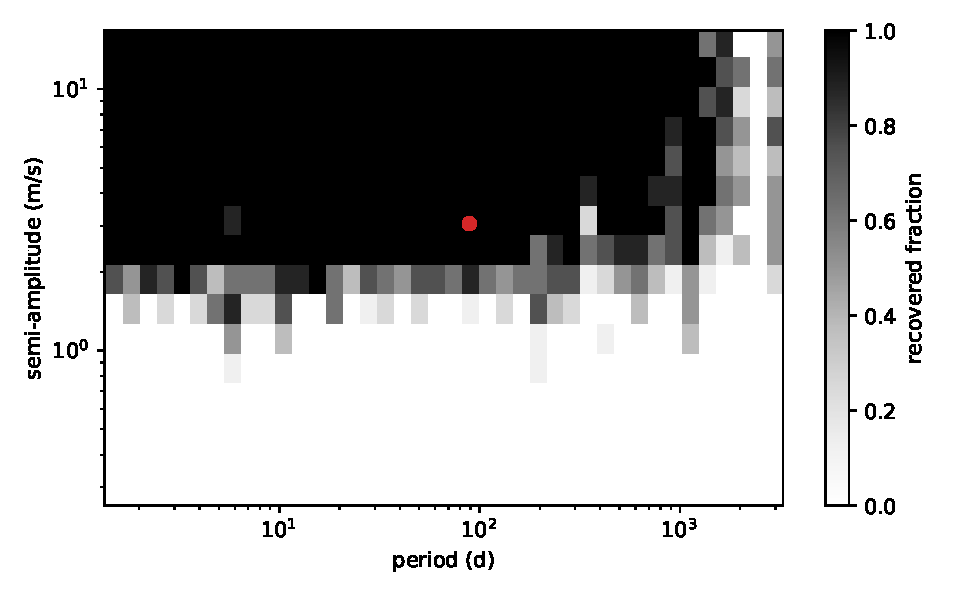
\includegraphics[width=0.8\textwidth]{detection_limits.pdf}
\caption{The fraction of circular orbits injected into the residuals of the HARPS and HIRES velocities
that are recovered, the highest peak of the residual periodogram within 2 per cent of the injected
period at a false-alarm level below $10^{-3}$, eight phases at each period and semi-amplitude. The
planet is marked.}\label{fig:limits}
\end{figure}

\section{TESS}\label{sec:tess}

TESS observed HD\,71334 in five sectors. Its light varies by less than 75\,ppm in each, the
periodograms' highest peaks lying at 2.7 to 9.3\,d with semi-amplitudes of 14 to 73\,ppm and differing
from sector to sector, and box least squares~\cite{Kovacs2002} within 2 per cent of the period finds
no transit repeated
at a constant depth: the best box's two events, of four and six points, differ in depth by a factor of
3.6. The circular orbit's conjunctions, where a transit would fall, carried into the sectors with their
errors, all fall outside them (Table~\ref{tab:tess}). The conjunction nearest sector 8 comes
$6.3 \pm 2.3$\,d before it begins and the one nearest sectors 34 and 35 $6.1 \pm 2.7$\,d before sector
34 begins, and sectors 61 and 88 lie 30 and 17\,d from the nearest. TESS has therefore not observed a
conjunction, and whether the planet transits is open. Its transit probability is 1.3 per cent; a
central transit would last 8.7\,h, and a planet of 4 to 6 Earth radii would take 1\,200 to 2\,800\,ppm
of the light. Table~\ref{tab:conjunctions} gives the conjunctions of the next two years; those of
2027 February and 2028 January fall when the star stands farthest from the Sun, and their errors of
four to five days grow by 0.067\,d with every orbit until new velocities shorten them.

\begin{table}[!htbp]
\centering
\caption{TESS's sectors of HD\,71334 and the planet's conjunctions on either side of each, from the
circular orbit, in BJD$-$2457000.}\label{tab:tess}
\begin{tabular}{c c r r}
\toprule
Sector & Dates & Conjunction before & Conjunction after \\
\midrule
8 & 2019 Feb 3--27 & $1511.7 \pm 2.3$ & $1600.6 \pm 2.3$ \\
34 & 2021 Jan 14--Feb 8 & $2222.9 \pm 2.7$ & $2311.8 \pm 2.8$ \\
35 & 2021 Feb 10--Mar 6 & $2222.9 \pm 2.7$ & $2311.8 \pm 2.8$ \\
61 & 2023 Jan 19--Feb 12 & $2934.2 \pm 3.2$ & $3023.1 \pm 3.3$ \\
88 & 2025 Jan 14--Feb 11 & $3645.5 \pm 3.7$ & $3734.4 \pm 3.8$ \\
\bottomrule
\end{tabular}
\end{table}

\begin{table}[!htbp]
\centering
\caption{The coming conjunctions of HD\,71334\,b from the circular orbit, with their errors, and the
Sun's distance from the star on each date.}\label{tab:conjunctions}
\begin{tabular}{r l r r}
\toprule
BJD & Date & Error (d) & Solar elongation \\
\midrule
2461356.8 & 2026 Nov 12 & 4.3 & $90^\circ$ \\
2461445.7 & 2027 Feb 9 & 4.3 & $133^\circ$ \\
2461534.6 & 2027 May 9 & 4.4 & $91^\circ$ \\
2461623.5 & 2027 Aug 5 & 4.4 & $48^\circ$ \\
2461712.4 & 2027 Nov 2 & 4.5 & $84^\circ$ \\
2461801.3 & 2028 Jan 30 & 4.6 & $132^\circ$ \\
\bottomrule
\end{tabular}
\end{table}

\section{Discussion}\label{sec:discussion}

HD\,71334\,b's minimum mass, $20.1 \pm 1.8$\,\Mearth, is a little above Neptune's 17. At 0.380\,au from
a star of 0.99\,\Lsun\ it receives 6.9 times the Earth's insolation, for an equilibrium temperature of
450\,K with no albedo: a warm Neptune on a circular orbit around a star much like the Sun, twice its age
and a little poorer in metals. Its true mass is its minimum mass divided by $\sin i$, and Gaia bounds the
largest: a companion of 0.1\,\Msun\ on this orbit would carry the star's photocentre around a 0.9-mas
ellipse every 89 days, which a single-star astrometric solution with a RUWE of 0.99~\cite{Lindegren2021}
leaves no room for.

The planet stood in the public record for two decades. Keck's velocities from 1997 and HARPS's from
2003 both hold it, and the joint record of 22 years fixes its period to 0.07\,d. Line-by-line
velocities measured from the archive's one-dimensional spectra inherit each spectrum's wavelength
calibration, and the pipeline calibrated some spectra with a ThAr exposure months old. Against a
signal of 3\,\ms, a dozen such spectra are enough to move a periodogram's highest peak to a one-year
alias, and they have to be set aside, or their drift restored, before an alias is read from
line-by-line velocities.

\section{Conclusion}\label{sec:conclusion}

HD\,71334, a quiet G2.5 dwarf of 0.93\,\Msun\ at 39.2\,pc, about 10\,Gyr old, hosts a planet of at least
20\,\Mearth\ on a circular 88.91-day orbit at 0.38\,au, read from 67 nights of public HARPS velocities
and 34 of Keck's over 22 years. The signal stands in three reductions of the HARPS spectra and in the
activity-quiet lines alone, keeps its amplitude and phase across the data, appears in Keck's velocities
at HARPS's phase, has no counterpart in eight activity indicators, and outweighs both one-year aliases.
TESS has not yet observed one of its conjunctions; photometry at the predicted times would tell
whether it transits, and new velocities would sharpen those times and test the residual at 40.7\,d.

\section*{Acknowledgements}

Based on data obtained from the ESO Science Archive Facility, on HARPS-RVBank, and on DACE, the Data \&
Analysis Center for Exoplanets, a facility of the University of Geneva and a platform of the Swiss
National Centre of Competence in Research PlanetS. The HIRES velocities are the California Legacy
Survey's, from the W. M. Keck Observatory. This work has made use of data from the European Space Agency
mission Gaia, processed by the Gaia Data Processing and Analysis Consortium, funded by national
institutions, in particular the institutions participating in the Gaia Multilateral Agreement; and of
the TESS mission, funded by NASA's Science Mission Directorate. The velocities, tests and orbits were
computed with orbitlight's planets mode.

\begin{thebibliography}{99}\small\raggedright
\setlength{\itemsep}{1pt}

\bibitem{Howard2010}
A.~W. Howard et al., The occurrence and mass distribution of close-in super-Earths, Neptunes, and
Jupiters, \emph{Science} \textbf{330}, 653 (2010).

\bibitem{Trifonov2020}
T.~Trifonov et al., Public HARPS radial velocity database corrected for systematic errors,
\emph{Astron. Astrophys.} \textbf{636}, A74 (2020).

\bibitem{Zechmeister2018}
M.~Zechmeister et al., Spectrum radial velocity analyser (SERVAL). High-precision radial velocities and
two alternative spectral indicators, \emph{Astron. Astrophys.} \textbf{609}, A12 (2018).

\bibitem{Rosenthal2021}
L.~J. Rosenthal et al., The California Legacy Survey. I. A catalog of 178 planets from precision radial
velocity monitoring of 719 nearby stars over three decades, \emph{Astrophys. J. Suppl. Ser.}
\textbf{255}, 8 (2021).

\bibitem{Adams1979}
D.~Adams, \emph{The Hitchhiker's Guide to the Galaxy} (Pan Books, London, 1979).

\bibitem{LoCurto2015}
G.~Lo Curto et al., HARPS gets new fibres after 12 years of operations, \emph{The Messenger}
\textbf{162}, 9 (2015).

\bibitem{Bouchy2001}
F.~Bouchy, F.~Pepe and D.~Queloz, Fundamental photon noise limit to radial velocity measurements,
\emph{Astron. Astrophys.} \textbf{374}, 733 (2001).

\bibitem{Artigau2022}
\'E.~Artigau et al., Line-by-line velocity measurements: an outlier-resistant method for precision
velocimetry, \emph{Astron. J.} \textbf{164}, 84 (2022).

\bibitem{Ricker2015}
G.~R. Ricker et al., Transiting Exoplanet Survey Satellite, \emph{J. Astron. Telesc. Instrum. Syst.}
\textbf{1}, 014003 (2015).

\bibitem{Lightkurve2018}
Lightkurve Collaboration, Lightkurve: Kepler and TESS time series analysis in Python, Astrophysics
Source Code Library, ascl:1812.013 (2018).

\bibitem{GaiaDR3}
Gaia Collaboration, A.~Vallenari et al., Gaia Data Release 3. Summary of the content and survey
properties, \emph{Astron. Astrophys.} \textbf{674}, A1 (2023).

\bibitem{Creevey2023}
O.~L. Creevey et al., Gaia Data Release 3. Astrophysical parameters inference system (Apsis). I. Methods
and content overview, \emph{Astron. Astrophys.} \textbf{674}, A26 (2023).

\bibitem{Noyes1984}
R.~W. Noyes et al., Rotation, convection, and magnetic activity in lower main-sequence stars,
\emph{Astrophys. J.} \textbf{279}, 763 (1984).

\bibitem{Mamajek2008}
E.~E. Mamajek and L.~A. Hillenbrand, Improved age estimation for solar-type dwarfs using
activity-rotation diagnostics, \emph{Astrophys. J.} \textbf{687}, 1264 (2008).

\bibitem{Zechmeister2009}
M.~Zechmeister and M.~K\"urster, The generalised Lomb-Scargle periodogram. A new formalism for the
floating-mean and Keplerian periodograms, \emph{Astron. Astrophys.} \textbf{496}, 577 (2009).

\bibitem{Baluev2008}
R.~V. Baluev, Assessing the statistical significance of periodogram peaks, \emph{Mon. Not. R. Astron.
Soc.} \textbf{385}, 1279 (2008).

\bibitem{Schwarz1978}
G.~Schwarz, Estimating the dimension of a model, \emph{Ann. Statist.} \textbf{6}, 461 (1978).

\bibitem{Dawson2010}
R.~I. Dawson and D.~C. Fabrycky, Radial velocity planets de-aliased: a new, short period for super-Earth
55 Cnc e, \emph{Astrophys. J.} \textbf{722}, 937 (2010).

\bibitem{ForemanMackey2013}
D.~Foreman-Mackey, D.~W. Hogg, D.~Lang and J.~Goodman, emcee: the MCMC hammer, \emph{Publ. Astron. Soc.
Pac.} \textbf{125}, 306 (2013).

\bibitem{terBraak2006}
C.~J.~F. ter Braak, A Markov chain Monte Carlo version of the genetic algorithm Differential Evolution:
easy Bayesian computing for real parameter spaces, \emph{Stat. Comput.} \textbf{16}, 239 (2006).

\bibitem{Lucy1971}
L.~B. Lucy and M.~A. Sweeney, Spectroscopic binaries with circular orbits, \emph{Astron. J.}
\textbf{76}, 544 (1971).

\bibitem{Kovacs2002}
G.~Kov\'acs, S.~Zucker and T.~Mazeh, A box-fitting algorithm in the search for periodic transits,
\emph{Astron. Astrophys.} \textbf{391}, 369 (2002).

\bibitem{Lindegren2021}
L.~Lindegren et al., Gaia Early Data Release 3. The astrometric solution, \emph{Astron. Astrophys.}
\textbf{649}, A2 (2021).

\bibitem{vanLeeuwen2007}
F.~van Leeuwen, Validation of the new Hipparcos reduction, \emph{Astron. Astrophys.} \textbf{474}, 653
(2007).

\bibitem{Huang2022}
C.~Huang, D.~R. Rice and J.~H. Steffen, MAGRATHEA: an open-source spherical symmetric planet interior
structure code, \emph{Mon. Not. R. Astron. Soc.} \textbf{513}, 5256 (2022).

\end{thebibliography}

\end{document}
